\documentclass{article}
\usepackage{cite, hyperref}

\title{contiBAIT: Improving Genome Assemblies Using Strand-seq Data}
\author{Kieran O'Neill, Mark Hills and Mike Gottlieb}

%\VignetteIndexEntry{flowBi}ngit 

\usepackage{Sweave}
\begin{document}
\Sconcordance{concordance:contiBAIT.tex:/data/ContiBAIT/vignettes/contiBAIT.Rnw:%
1 8 1 1 0 31 1 1 4 3 0 1 4 3 0 1 3 4 0 1 2 2 1 1 3 11 0 1 4 2 0 2 1 3 0 %
1 2 4 1 1 4 6 0 1 2 4 1 1 4 3 0 1 1 6 0 1 2 5 1 1 2 1 0 1 1 2 2 2 1 1 2 %
10 0 1 1 15 0 1 2 2 1 1 2 4 0 1 2 6 1}

\setkeys{Gin}{width=0.75\textwidth}
\setkeys{Gin}{height=0.75\textwidth}

\maketitle
\begin{center}
{\tt koneill@bcgsc.ca}
\end{center}

\textnormal{\normalfont}

\tableofcontents
\newpage



\section{Licensing}
Under the Two-Clause BSD License, you are free to use and redistribute this software.

\section{Introduction}
Strand-seq is a method for determining template strand inheritance in single cells.
When strand-seq data are collected for many cells from the same organism, spatially close genomic regions show similar patterns of template strand inheritance.
ContiBAIT allows users to leverage this property to carry out three tasks to improve draft genomes. Firstly, in assemblies made up entirely of contigs or scaffolds not yet assigned to chromosomes, these contigs can be clustered into chromosomes. Secondly, in assemblies wherein scaffolds have been assigned to chromosomes, but not yet placed on those chromosomes, those scaffolds can be placed in order relative to each other. Thirdly, for assemblies at the chromosome stage, where scaffolds are ordered and separated by many unbridged sequence gaps, the orientation of these sequence gaps can be found.  

All three of these tasks can be run in parallel, taking contig-stage assemblies and ordering all fragments first to chromosomes, then within chromosomes while simultaneously determining the relative orientation of each fragment. This vignette will outline some specific functions of contiBAIT, and is comparible to the contiBAIT() master function included in this package that will perform the same sequence of function calls outlined below.

\section{Input}
ContiBAIT requires input in BAM format. Multiple BAM files are required for analysis, so ContiBAIT specifically calls for users to identify a BAM directory in which to analyse. Sorted BAM files will speed up analysis. 
 
\begin{Schunk}
\begin{Sinput}
> # Read in BAM files. Path denotes location of the BAM files.
> # Returns a vector of file locations
> 
> library(contiBAIT)
> bamFileList <- list.files(
+ path=file.path(system.file(package='contiBAIT'), 'extdata'),
+ pattern=".bam$",
+ full.names=TRUE)
\end{Sinput}
\end{Schunk}

The example data provided by contiBAIT is from a human blood sample and has been aligned to GRCh38/hg38.  Since this assembly is already complete, we must first split this genome into chunks to simulate a contig-stage assembly. To do this we need to extract information on the assembly the bam file is aligned to by creating a chromosome table instance, then splitting this table.

\subsection{\textit{Creating a chromosome table instance}}

The example data provided with the contiBAIT package is derived from GRCh38/hg38 data (only aligned to all autosomes and allosomes; no alternative locations or contigs were included). To subset these data, and for further downstream analysis, a GRanges chromosome table instance can be made, representing the contig name and length. This is generated with makeChrTable, where the resulting object is similar to the header portion of a BAM file. Note a meta column with a name formed of the contig and start and end locations is generated for downstream workflows.

\begin{Schunk}
\begin{Sinput}
> # build chr table from BAM file in bamFileList
> 
> exampleChrTable <- makeChrTable(bamFileList[1]) 
> exampleChrTable
\end{Sinput}
\begin{Soutput}
ChrTable object with 24 ranges and 1 metadata column:
       seqnames         ranges strand   |             name
          <Rle>      <IRanges>  <Rle>   |      <character>
   [1]     chr1 [0, 249250621]      *   | chr1:0-249250621
   [2]     chr2 [0, 243199373]      *   | chr2:0-243199373
   [3]     chr3 [0, 198022430]      *   | chr3:0-198022430
   [4]     chr4 [0, 191154276]      *   | chr4:0-191154276
   [5]     chr5 [0, 180915260]      *   | chr5:0-180915260
   ...      ...            ...    ... ...              ...
  [20]    chr20 [0,  63025520]      *   | chr20:0-63025520
  [21]    chr21 [0,  48129895]      *   | chr21:0-48129895
  [22]    chr22 [0,  51304566]      *   | chr22:0-51304566
  [23]     chrX [0, 155270560]      *   | chrX:0-155270560
  [24]     chrY [0,  59373566]      *   |  chrY:0-59373566
  -------
  seqinfo: 24 sequences from an unspecified genome; no seqlengths
\end{Soutput}
\end{Schunk}

\subsection{\textit{Splitting a chromosome table instance}}

We can also split the above chromosome table instance into 1 Mb fragments. This subdivision isn't just for testing purposes. For chromosome- and contig-stage assemblies with very large fragments, subdividing the data into bins can help identify chimeric fragments and misorientations. Some assemblies have a large degree of misorientations or chimerism in the data, and subdividing them aids in clustering these fragments.  For example, if a region is misoriented within a contig, the strand state will change in this region, skewing this contig toward a WC call in every library. However, while fragmenting can improve the overall number of contigs included in analysis and improve clustering, as the fragments get further subdivided, the number of reads used to make strand state calls decreases, and the probability of there being insufficient reads to make an accurate call increases.  Note the following divided chromosome table can be used with the filter argument in strandSeqFreqTable to generate a sub-divided table.

\begin{Schunk}
\begin{Sinput}
> exampleDividedChr <- makeChrTable(bamFileList[1], splitBy=1000000)
> exampleDividedChr
\end{Sinput}
\begin{Soutput}
ChrTable object with 3089 ranges and 1 metadata column:
         seqnames               ranges strand   |                   name
            <Rle>            <IRanges>  <Rle>   |            <character>
     [1]     chr1   [      0, 1001006]      *   |         chr1:0-1001006
     [2]     chr1   [1001007, 2002012]      *   |   chr1:1001007-2002012
     [3]     chr1   [2002013, 3003019]      *   |   chr1:2002013-3003019
     [4]     chr1   [3003020, 4004025]      *   |   chr1:3003020-4004025
     [5]     chr1   [4004026, 5005032]      *   |   chr1:4004026-5005032
     ...      ...                  ...    ... ...                    ...
  [3085]     chrY [54341909, 55348239]      *   | chrY:54341909-55348239
  [3086]     chrY [55348240, 56354571]      *   | chrY:55348240-56354571
  [3087]     chrY [56354572, 57360903]      *   | chrY:56354572-57360903
  [3088]     chrY [57360904, 58367234]      *   | chrY:57360904-58367234
  [3089]     chrY [58367235, 59373566]      *   | chrY:58367235-59373566
  -------
  seqinfo: 24 sequences from an unspecified genome; no seqlengths
\end{Soutput}
\end{Schunk}

\subsection{\textit{Splitting a chromosome table based on strand state changes}}
A change in strand state within a contig can represent a number of things. At it's simplest, it could represent a sister chromatid exchange switching the templates in that particular cell. In cases where the same location is a site of recurrent strand state changes, the more likely explanation is that the fragment is chimeric or has a misorientation within it. contiBAIT allows users to cut contigs at these locations to allow for better clustering. The most likely site of incorrectly oriented or placed fragments is at unbridged or bridged gap regions. A function is included that allows us to look for overlaps between recurrent strand state changes and gap regions.

\begin{Schunk}
\begin{Sinput}
> library(rtracklayer)
> # Download GRCh38/hg38 gap track from UCSC
> gapFile <- import.bed("http://genome.ucsc.edu/cgi-bin/hgTables?hgsid=465319523_SLOtFPExny48YZFaXBh4sSTzuMcA&boolshad.hgta_printCustomTrackHeaders=0&hgta_ctName=tb_gap&hgta_ctDesc=table+browser+query+on+gap&hgta_ctVis=pack&hgta_ctUrl=&fbQual=whole&fbUpBases=200&fbDownBases=200&hgta_doGetBed=get+BED")
> # Create fake SCE file with four regions that overlap a gap
> sceFile <- GRanges(rep('chr4',4), 
+ IRanges(c(1410000, 1415000, 1420000, 1425000), 
+ c(1430000, 1435000, 1430000, 1435000)))
> overlappingFragments <- mapGapFromOverlap(sceFile,
+  gapFile, 
+  exampleChrTable, 
+  overlapNum=4)
> show(overlappingFragments)
\end{Sinput}
\begin{Soutput}
ChrTable object with 26 ranges and 1 metadata column:
       seqnames               ranges strand   |                 name
          <Rle>            <IRanges>  <Rle>   |          <character>
   [1]     chr1 [      0, 249250621]      *   |     chr1:0-249250621
   [2]     chr2 [      0, 243199373]      *   |     chr2:0-243199373
   [3]     chr3 [      0, 198022430]      *   |     chr3:0-198022430
   [4]     chr4 [      0,   1429358]      *   |       chr4:0-1429358
   [5]     chr4 [1429359,   1434206]      *   | chr4:1429359-1434206
   ...      ...                  ...    ... ...                  ...
  [22]    chr20       [0,  63025520]      *   |     chr20:0-63025520
  [23]    chr21       [0,  48129895]      *   |     chr21:0-48129895
  [24]    chr22       [0,  51304566]      *   |     chr22:0-51304566
  [25]     chrX       [0, 155270560]      *   |     chrX:0-155270560
  [26]     chrY       [0,  59373566]      *   |      chrY:0-59373566
  -------
  seqinfo: 64 sequences from an unspecified genome; no seqlengths
\end{Soutput}
\end{Schunk}

What is returned is a GRanges chromosome table instance where the gap that is coincident with the recurrent strand state change has split that contig into two smaller fragments. Note the example table now has 25 fragments as chr4 has been split.

\subsection{\textit{Creating a strandFreqMatrix instance}}

To read in BAM files into ContiBAIT, create a strandFreMatrix instance by calling strandSeqFreqTable().  This program will read each BAM file, calculate the ratio of W and C reads, and return this value along with the total number of reads used to make the call. Note, we will use the GRanges divided chromosome table to simultaneously cut the assembly into 1 Mb fragments.  By default duplicate reads are removed, a minimal mapping quality of 0 is used and the function expects to see paired end data. Because of the way BAM files store strand information, it is important to ensure that the pairedEnd parameter is correctly set. A warning will be issued if single-end data is run as if it is paired-end.

\begin{Schunk}
\begin{Sinput}
> # Create a strandFreqTable instance 
> 
> strandFrequencyList <- strandSeqFreqTable(bamFileList, 
+ filter=exampleDividedChr,
+ qual=10, 
+ pairedEnd=FALSE,
+ BAITtables=TRUE)
\end{Sinput}
\end{Schunk}

This returns a list of two data.frames if the BAITtables argument is set to FALSE, or four if it is set to TRUE.  The first data.frame consists of a strand state frequency, calculated by taking the number of Watson (- strand) reads, subtracting the number of Crick (+ strand) reads, and dividing by the total number of reads.  These values range from -1 (entirely Watson reads) through to 1 (entirely Crick reads).  The second data.frame consists of the absolute number of reads covering the contig. This is used in thresholding the data, and in weighting the accuracy of calls in subsequent orderings. Note that the fewer reads used to make a strand call, the less accurate that call will be. In the absence of background reads, WC regions will follow a binomial distribution. If we assume any contigs with <-0.8 are WW, and >0.8 are CC (this is the default strandTableThreshold parameter used in preprocessStrandTable), then there is a probability of 0.044 that the strand state call is incorrect. As such we exclude calls that are made with fewer than 10 reads. Increasing this number will make calls more accurate, but will reduce the number of contigs included in analysis. Since the contigs are weighted based on read density during clustering, a minimum of 10 reads to support a strand call provides a good balance between accuracy and inclusion.

\begin{Schunk}
\begin{Sinput}
> # Returned list consisting of two data.frames
> strandFrequencyList
\end{Sinput}
\begin{Soutput}
$strandTable
A matrix of strand frequencies for 145 contigs over 35 libraries.

$countTable
A matrix of read counts for 145 contigs over 35 libraries.

$WatsonReads
A matrix of read counts for 3089 contigs over 35 libraries.

$CrickReads
A matrix of read counts for 3089 contigs over 35 libraries.
\end{Soutput}
\begin{Sinput}
> # Exclude frequencies calculated from
> # contigs with less than 10 reads
> 
> exampleStrandFreq <- strandFrequencyList[[1]]
> exampleReadCounts <- strandFrequencyList[[2]]
> exampleStrandFreq[which(exampleReadCounts < 10)] <- NA 
\end{Sinput}
\end{Schunk}

Additional information can be found on the help page for strandSeqFreqTable including all parameters.\\

The quality of the libraries, specifically whether the files being analysed appear to show the expected distributions of directional reads, can be assessed with plotWCdistributions.  In a diploid organism, there is an expectation that chromosomes will be derived from either two Watson homologues, one Watson and one Crick homologue, or two Crick homologues in a Mendelian 1:2:1 ratio.  In Strand-seq data, this will mean about 1/4 of the contigs will only have Watson reads mapping to them, and have a strand state frequency of -1, 1/4 of the contigs will only have Crick reads mapping to them, and have a strand state frequency of +1, and 1/2 of the contigs will have an approximately even mix of Watson and Crick reads (based on a binomial distribution of sampling).  plotWCDistribution generates boxplots for different strand state frequencies and models the expected distribution (blue line). The average called WW or CC contigs are shown in green, and should match closely with the expected distribution line.

\begin{Schunk}
\begin{Sinput}
> # Assess the quality of the libraries being analysed
> plotWCdistribution(exampleStrandFreq)
\end{Sinput}
\end{Schunk}
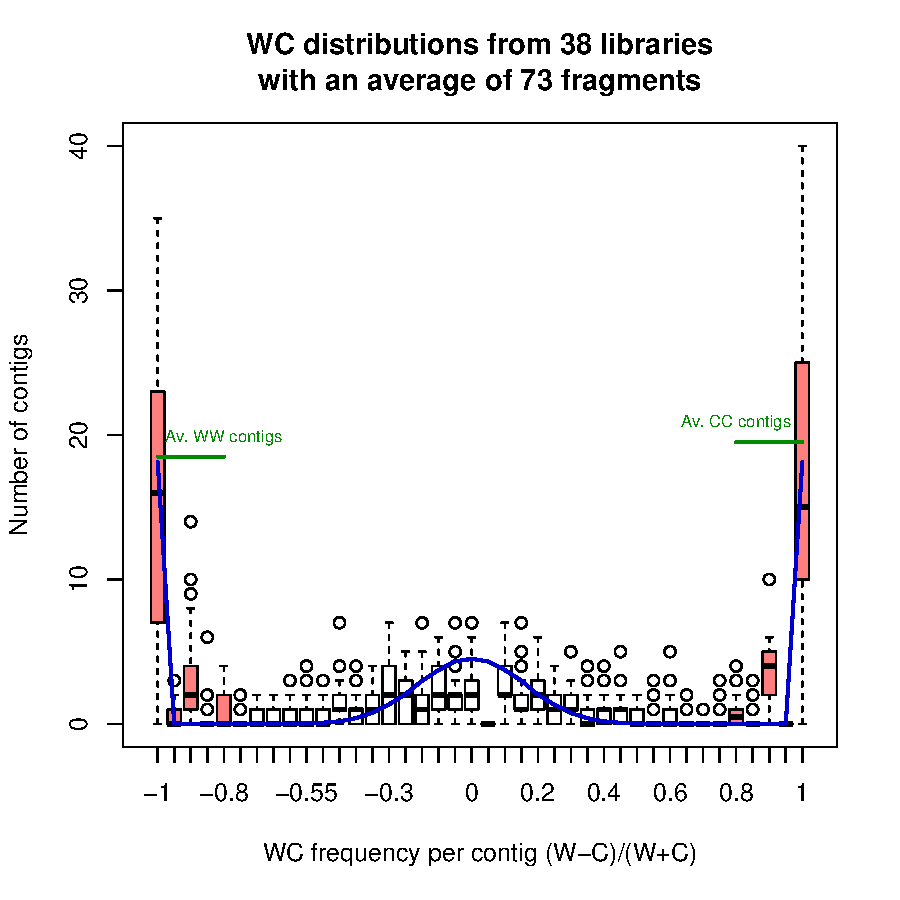
\includegraphics{contiBAIT-strandSeqFreqTableExamplec}

\section{Creating a strand state matrix}

The returned list of strandSeqFreqTable can be converted to a strand state matrix that makes a contig-wide call on the overall strand state based on the frequencies of Watson and Crick reads. The function removes BAM files that either contain too few reads to make accurate strand calls or are not strand-seq libraries (i.e. every contig contains approximately equal numbers of + and - reads). Conversely the function removes contigs that either contain too few reads, or always contain roughly equal numbers of + and - reads.  More details on the parameters can be found in the function documentation.  The function returns a similar data.frame to strandSeqFreqTable, but with the frequencies converted to strand calls: 1 is a homozygous Watson call (by default, a frequency less than -0.8, but this can be changed with the filterThreshold argument), 2 is a heterozygous call (a frequency between -0.8 and 0.8 by default) and 3 is a homozygous Crick call (by default, a frequency above 0.8).  These factors can then be used to cluster similar contigs together.\\


\begin{Schunk}
\begin{Sinput}
> # Convert strand frequencies to strand calls.
> 
> exampleStrandStateMatrix <- preprocessStrandTable(
+ exampleStrandFreq, 
+ lowQualThreshold=0.8)
> exampleStrandStateMatrix[[1]]
\end{Sinput}
\begin{Soutput}
A strand state matrix for 76 contigs over 35 libraries.
\end{Soutput}
\end{Schunk}

\section{Clustering contigs into chromosomes}

clusterContigs utilizes a custom algorithm to cluster all fragments together that share a similar strand state across multiple cells.  For example, if two contigs are adjacent on the same chromosome, then they will inherit the same strand state in every cell that is analyzed.  It is important to note however that the relative directionality of any two fragments within an assembly is unknown. Contigs which belong on the same chromosome but are in different orientations will display as complete opposites; every library where one contig is homozygous Watson will have the other contig as homozygous Crick.  However, heterozygous contigs (where chromosomes inherited one Watson template and one Crick template), will not be mirrored, with one contig being "WC", while the other will be "CW". As such, by default the function performs clustering between homozygous calls (WW or CC treated the same) and heterozygous calls (WC) to identify contigs that belong together despite their misorientation status with respect to each other. Using the clusterBy='homo' option will perform the clustering just between WW and CC calls (ignoring WC calls) and misoriented fragments from the same chromosome will cluster into different linkage groups. Once clustered, the misorientated fragments are identified in each linkage group using reorientAndMergeLGs. Since chromosome orientation cannot be determined by sequence alone, the largest sub-group is arbitrarily considered "+", while the smaller group is considered "-". The product of this function is a list where the first element is a StrandStateMatrix instance that has been correctly oriented, the second element is a data.frame of contigs and orientations, and the third element is a recomputed LinkageGroupList that merges groups that were previously discordant based on misorientation status. This merger occurs by computing a consensus strand state across libraries within each linkage group and comparing them.   Note for the purposes of this example, we are using the argument randomise=FALSE to ensure conformity of the vignette when running sweave. Randomisation is recommended for most applications and is set to TRUE by default.

\begin{Schunk}
\begin{Sinput}
> exampleWCMatrix <- exampleStrandStateMatrix[[1]]
> clusteredContigs <- clusterContigs(exampleWCMatrix, randomise=FALSE)
> reorientedMatrix <- reorientAndMergeLGs(clusteredContigs,
+  exampleWCMatrix)
> exampleLGList <- reorientedMatrix[[3]]
> exampleLGList
\end{Sinput}
\begin{Soutput}
A linkage group list containing 5 linkage groups.

  NumberOfContigs
1              19
2              19
3              19
4              18
5               1
\end{Soutput}
\begin{Sinput}
> exampleLGList[[1]]
\end{Sinput}
\begin{Soutput}
 [1] "chr3:3000340-4000452"     "chr3:30003399-31003511"  
 [3] "chr3:6000680-7000792"     "chr3:190021525-191021637"
 [5] "chr3:160018126-161018238" "chr3:130014727-131014840"
 [7] "chr3:150016993-151017105" "chr3:50005664-51005777"  
 [9] "chr3:1000113-2000226"     "chr3:10001133-11001245"  
[11] "chr3:110012462-111012574" "chr3:40004532-41004644"  
[13] "chr3:20002266-21002378"   "chr3:100011329-101011441"
[15] "chr3:170019259-171019371" "chr3:70007930-71008042"  
[17] "chr3:120013595-121013707" "chr3:60006797-61006910"  
[19] "chr3:80009063-81009175"  
\end{Soutput}
\end{Schunk}


The clusterContigs function generates a list of linkage groups consisting of all the clustered contigs.  After reorientation and merging, all contigs within the linkage groups are highly similar, while the contigs between linkage groups are highly dissimilar.  The similarity between linkage groups can be visualized using plotLGDistances.

\begin{Schunk}
\begin{Sinput}
> plotLGDistances(exampleLGList, exampleWCMatrix)
\end{Sinput}
\end{Schunk}
\includegraphics{contiBAIT-clusterContigsExampleb}


While the similarity within linkage groups can be visualized using plotLinkageGroup (here, the first linkage group is used for creating this heatmap). Note, side by side comparisons of linkage group members can be performs with multiple lg options (e.g. lg=1:2 will plot the first two linkage groups, lg=c(1,4) will plot the first and forth etc.).

\begin{Schunk}
\begin{Sinput}
> plotLGDistances(exampleLGList, exampleWCMatrix, lg=1)
\end{Sinput}
\end{Schunk}
\includegraphics{contiBAIT-clustercontigsExamplec}


\section{Ordering contigs within chromosomes}

With contigs clustered to chromosomes, we can then order them within chromosomes. Just as meiotic recombination shuffles loci and allows genetic distances between them to be determined, sister chromatid exchanges (SCE) events reshuffle templates, and similarly allow us to infer a linkage distance. We have employed a greedy algorithm to do this, but have an argument allowing a TSP solution as an alternative. Contigs are ordered by similarity across libraries, then by contig name. Contigs that are zero distance apart (ie have no SCE events between them and are therefore unordered) are returned in contig name order. The output is split into sub-linkage groups, so Linkage group 1 will be split into a number of groups depending on the number of SCE events that occur within the chromosome. The output will be an S4 object of type contigOrdering.

\begin{Schunk}
\begin{Sinput}
> contigOrder <- orderAllLinkageGroups(exampleLGList,
+ exampleWCMatrix,
+ exampleStrandFreq,
+ exampleReadCounts,
+ whichLG=1,
+ saveOrdered=TRUE)
> contigOrder[[1]]
\end{Sinput}
\begin{Soutput}
A matrix of 1 LGs split into 12 sub-groups from 19 ordered fragments.

 LG1.1 LG1.10 LG1.11 LG1.12  LG1.2  LG1.3  LG1.4  LG1.5  LG1.6  LG1.7  LG1.8 
     1      1      2      1      2      3      2      1      3      1      1 
 LG1.9 
     1 
\end{Soutput}
\end{Schunk}
\includegraphics{contiBAIT-orderAllLinkageGroupsExample}

If the assembly is mostly complete and you wish to compare the actual location of the fragments in the assembly you're working with against the output of orderAllLinkageGroups, contiBAIT has the built in plotContigOrder function. This assumes that the contig name from the contigOrdering object is in a format of chr:start-end.

\begin{Schunk}
\begin{Sinput}
> plotContigOrder(contigOrder[[1]])
\end{Sinput}
\end{Schunk}
\includegraphics{contiBAIT-orderAllLinkageGroupsExampleb}

Alternatively, all contigs can be ordered simultaneously by omitting the whichLG argument. If saveOrdered is set to TRUE, plots will be generated for every linkage group.  By ordering all of the linkage groups we can proceed to create BED files of these data for the new assemblies.

\begin{Schunk}
\begin{Sinput}
> contigOrderAll <- orderAllLinkageGroups(exampleLGList,
+ exampleWCMatrix,
+ exampleStrandFreq,
+ exampleReadCounts)
> contigOrderAll[[1]]
\end{Sinput}
\begin{Soutput}
A matrix of 5 LGs split into 14 sub-groups from 76 ordered fragments.

 LG1.1 LG1.10 LG1.11 LG1.12  LG1.2  LG1.3  LG1.4  LG1.5  LG1.6  LG1.7  LG1.8 
     1      1      2      1      2      3      2      1      3      1      1 
 LG1.9  LG2.1 LG2.10 LG2.11 LG2.12 LG2.13 LG2.14  LG2.2  LG2.3  LG2.4  LG2.5 
     1      2      1      1      1      1      1      3      1      2      2 
 LG2.6  LG2.7  LG2.8  LG2.9  LG3.1 LG3.10 LG3.11 LG3.12  LG3.2  LG3.3  LG3.4 
     1      1      1      1      3      2      1      1      3      1      1 
 LG3.5  LG3.6  LG3.7  LG3.8  LG3.9  LG4.1 LG4.10 LG4.11  LG4.2  LG4.3  LG4.4 
     3      1      1      1      1      2      2      1      2      1      2 
 LG4.5  LG4.6  LG4.7  LG4.8  LG4.9  LG5.1 
     1      1      3      1      2      1 
\end{Soutput}
\end{Schunk}


\section{Checking order using BAIT ideograms}

It is possible to visually validate the ordering by creating ideogram plots of the data. The supplied test data comprises of reads from the first four chromosomes. Below is example code that will plot the second library from the output of strandSeqFreqTable. Note the third and forth elements of the strandFrequencyList are only generated if BAITtables is set to TRUE when running strandSeqFreqTable.  The plot below shows the location of the reads and highlights an SCE on chromosome 3. Note to only display the first library, we need to subset the strandReadMatrix and retain these as strandReadMatrix objects.

\begin{Schunk}
\begin{Sinput}
> # extract elements from strandSeqFreqTable list
> WatsonFreqList <- strandFrequencyList[[3]]
> CrickFreqList <- strandFrequencyList[[4]]
> # subset elements to only analyze one library
> singleWatsonLibrary <- StrandReadMatrix(WatsonFreqList[,2, drop=FALSE])
> singleCrickLibrary <- StrandReadMatrix(CrickFreqList[,2, drop=FALSE]) 
> # Run ideogram plotter
> ideogramPlot(singleWatsonLibrary,
+ singleCrickLibrary,
+ exampleDividedChr)
\end{Sinput}
\end{Schunk}
\includegraphics{contiBAIT-ideogramExample}

If chromosome builds are not complete (and so each contig has not been assigned a chromosome in the chrTable instance), these ideograms can be plotted using only the represented fragments in the order given to the function from the orderedContig object generated from orderAllLinkageGroups.  Here we will use the orderedContig object representing all 4 linkage groups.

\begin{Schunk}
\begin{Sinput}
> ideogramPlot(singleWatsonLibrary,
+ singleCrickLibrary,
+ exampleDividedChr,
+ orderFrame=contigOrderAll[[1]])
\end{Sinput}
\end{Schunk}
\includegraphics{contiBAIT-ideogramExampleb}

Alternatively, all libraries can be compared side by side for a single chromosome. Because this will print to multiple pages, the showPage option can be used to limit the output to a user=specified page. Here we will use the orderedContig object representing just one linkage group.

\begin{Schunk}
\begin{Sinput}
> ideogramPlot(WatsonFreqList,
+ CrickFreqList,
+ exampleDividedChr,
+ orderFrame=contigOrder[[1]],
+ plotBy='chr',
+ showPage=1)
\end{Sinput}
\end{Schunk}
\includegraphics{contiBAIT-ideogramExamplec}


\section{Writing out to a BED file}
This file can be passed to bedtools along with the original (draft) reference genome to create a new FASTA file containing the assembled genome. the writeBed function requires a chrTable of class ChrTable with which to extract the contig names and locations, the orientation information derived from reorientLinkageGroups to populate the strand column, the library weight to populate the score column, and an object of type ContigOrdering to invoke the actual order of fragments.  A fileName can be supplied, or the default is used. BED files will be written to the working directory

\begin{Schunk}
\begin{Sinput}
> writeBed(exampleDividedChr,
+ reorientedMatrix[[2]],
+ contigOrder[[1]])
\end{Sinput}
\end{Schunk}

\newpage
\section{Additional plotting functions}

Using a chromosome table instance, comparisons can be made between the portion of contigs that are included in the analysis verses those that are excluded based on either poor coverage or non-Strand-seq patterning. The code below generates a box plot of contig sizes that are included in the analysis. Note, since sample data are uniform 1 Mb framgents, the box plot does not deviate from the median.  The example bam files contain reads from 76 separate 1 Mb fragments from chromsomes 1, 2, 3, and 4.  Since the assembly is >3 Gb in size, only a few percent of the assembly will be included in our analysis.

\begin{Schunk}
\begin{Sinput}
> makeBoxPlot(exampleDividedChr, exampleLGList)
\end{Sinput}
\end{Schunk}
\includegraphics{contiBAIT-makeChrTableExamplec}

\newpage
Furthermore we can determine the proportion of assembly fragments in each linkage group in a barplot. If data are in the format chr:start-end, then each unique chromosome name will have a unique color. If data are not in this format, then each fragment will have a unique color.  Here, all fragments from chr1 will be colored differently to fragments from chr2, etc.

\begin{Schunk}
\begin{Sinput}
> barplotLinkageGroupCalls(exampleLGList, exampleDividedChr)
\end{Sinput}
\end{Schunk}
\includegraphics{contiBAIT-makeChrTableExampled}

Note that if clustering did not occur correctly, some bars would be a mixture of colors.  While the above displays the proportion of fragments from one chromosome that has clustered into each linkage group, but omitting the by='chr' parameter, the plot changes to the proportion of linkage groups within each chromosome.

\newpage

\section{Flow diagram}
Here is the basic functionality of the contiBAIT package.  The input BAM file(s) and output BED file are displayed in the grey ovals. All plotting functions are shown in blue hexagons and all analysis functions are in white boxes.


\setkeys{Gin}{width=\textwidth}
\setkeys{Gin}{height=15cm}
\begin{center}

\includegraphics{contiBAIT-fig1}
\end{center}
\end{document}
